This section documents the validation of the Matrix Element method by measuring the 
$\WZ/ZZ$ cross-section. This part of the analysis was performed with the 
Spring11 MC corresponding to the EPS selections. 

We validate performance of our implementation of the Matrix Element technique by simultaneously measuring
$WZ$ and $ZZ$ cross-section in the zero jet bin. 
%in events with two-charged leptons and missing transverse energy.
After the preselection cuts, the only relevant background in the measurement is non-resonant $WW$ production.
Therefore, the main challenge is to discriminate $ZZ$ and $WZ$ events from $WW$.

In order to achieve this, we construct new Likelihood $LR_{ZZ+WZ}$, defined as:

\begin{equation}
\label{eqn:LRZZ}
LR_{ZZ+WZ} = \frac { P_{ZZ}+P_{WZ}} { P_{ZZ} + P_{WZ} + P_{WW} },
\end{equation}

where $P_{WZ}$ is evaluated with the assumption that the two charged leptons originated from a $Z$-boson, while the
$W$ decays leptonically but the lepton was not reconstructed. The distribution of LR$_{ZZ+WZ}$ for data and the predicted 
backgrounds and signal is shown in figure \ref{fig:lrzz}. The shape of the distribution in data is well 
modeled by the simulation.

%%%%%%%%%%%%%%%%%%%%%%%%%%%%%%
\begin{figure}[!htbp]
\begin{center}
\subfigure[$ee$]{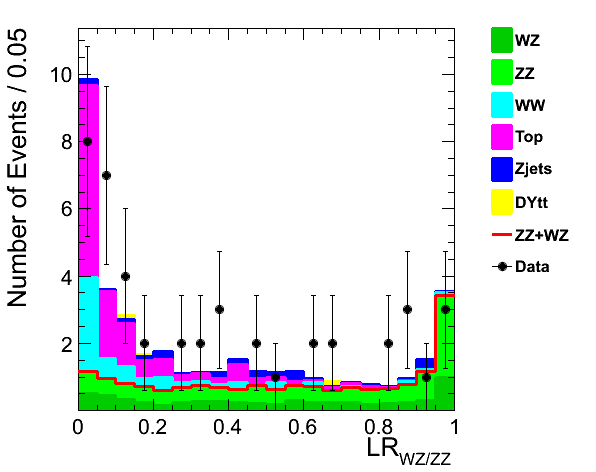
\includegraphics[width=0.47\textwidth]{figures/ME_WZZZ_mH0_ee_stack_lin.png}}
\subfigure[$\mu\mu$]{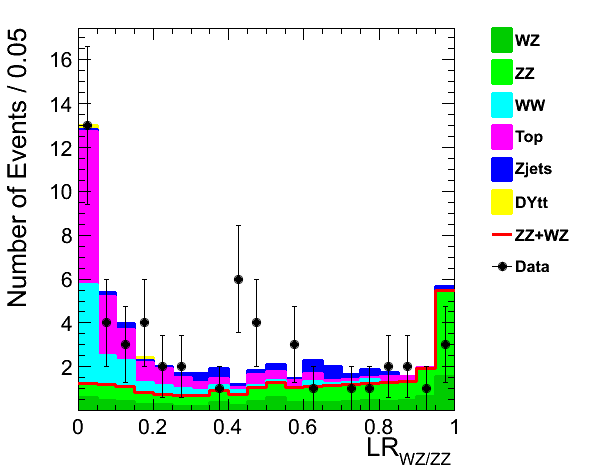
\includegraphics[width=0.47\textwidth]{figures/ME_WZZZ_mH0_mm_stack_lin.png}}
\caption{$LR_{ZZ+WZ}$ in 1092 pb$^{-1}$ of data compared to expected backgrounds and $ZZ+WZ$ signal.}
\label{fig:lrzz}
\end{center}
\end{figure}
%%%%%%%%%%%%%%%%%%%%%%%%%%%%%%

To accurately measure the cross section, we require a clean sample of signal events. 
This is achieved by selecting those events that 
that pass the requirement: $LR_{ZZ+WZ}>0.75$. 
The Expected yields for each process and the observed data count after this requirement
are shown in table \ref{tab:ZZWZselection}.

\begin{table}[!hbtp]
  \begin{center}
  \begin{tabular} {c|c|c}
 \hline
  Process & $\mu-\mu$ events  & $e-e$ events \\
  \hline
  \hline
  $WW$                  &  0.2 $\pm$  0.1 &  0.2 $\pm$   0.1 \\
  $tt + tW$             &  0.6 $\pm$  0.1 &  0.1 $\pm$   0.1 \\
  $Z  + jets$           &  0.8 $\pm$  0.1 &  0.5 $\pm$   0.1\\
  $Z\rightarrow \tau\tau$& 0.0 $\pm$  0.1 &  0.0 $\pm$   0.1\\
  \hline
  Total Background      &  1.6 $\pm$  0.2 &  0.8 $\pm$   0.2\\
  \hline
  $ZZ$                  &  7.7 $\pm$  0.2 &  4.8 $\pm$   0.1\\
  $WZ$                  &  3.5  $\pm$ 0.1 &  1.9 $\pm$   0.1\\
 \hline
  Total Signal          &  11.2 $\pm$ 0.3 &  6.7 $\pm$   0.2\\
 \hline
  Data                  &  9               &   9              \\
 \hline
  \end{tabular}

  \caption{Expected number of signal and background events for a data sample with an 
  integrated luminosity of 1.1 fb$^{-1}$ after applying the $LR_{ZZ/WZ}>0.75$ requirement. 
 Uncertainties are statistical only.}
   \label{tab:ZZWZselection}
  \end{center}
\end{table}

Assuming a 100$\%$ systematic unceratainty on the backgrounds, we estimate the $ZZ+WZ$ 
cross-section to be $22.8 \pm 3.5$ pb, which is in agreement with theoretical predictions of $26.2$ pb.

